The mathematical software systems to be integrated via the MitM approach have so far been computation-oriented, e.g., computer algebra systems.
Their API theories typically declare types and functions on these types (the latter including constants seen as nullary functions).
Even though database systems differ drastically from these in many respects, they are very similar at the MitM level: a mathematical database defines
\begin{compactitem}
 \item some types: each table's schema is essentially one type definition,
 \item many constants: each table entry is one constant of the corresponding type.
\end{compactitem}
Thus, we can reuse many of the same concepts.
In particular, the API theories must contain definitions of the database schemas. 

Apart from standard software engineering tasks, this leaves three conceptual problems we had to solve:
\begin{compactenum}[\bf P1]
\item Turn the database schemas and tables into \ommt theories and declarations. 
\item Lift data in \emph{physical} representation (as records of the
  underlying database) to \ommt object in \emph{semantic} representation.
\item Translate semantic queries to queries about physical representations so
  that they can be executed directly on the database without loading the entire theory into
  \mmt.
\end{compactenum}
We deal with \textbf{P1} in Section~\ref{sec:vt}, with \textbf{P2} in Section~\ref{sec:vt:codec}, and with \textbf{P3} in Section~\ref{sec:qmt}. 

In this paper, we focus on \lmfdb as an example, of which we give an overview in Section~\ref{sec:lmfdb}.
However, our methods are general enough to apply to many other mathematical databases such as OEIS, or findstat.

 \subsection{LMFDB Overview}\label{sec:lmfdb}
  \section{Example: The API and Structure of LMFDB}\label{sec:sota}

The ``L-Functions and Modular Forms Database'' (\lmfdb~\cite{lmfdb}) is a large database, storing among other mathematical objects several thousand L-Functions and curves along with their properties. 
Technically, it uses a MongoDB database with a Python web frontend. 
We use this as an example of a virtual theory. 
Before we go into this in more detail, we have a closer look at the structure and existing APIs to of \lmfdb.

\subsection{The Structure of LMFDB}\label{sec:sota:struct}

\lmfdb has several sub-databases, e.g., for elliptic curves or transitive groups. 
Within each of these, every object is stored as a single JSON record.
Figure~\ref{fig:lmfdbexample} shows an example: each property of this JSON object corresponds to a property of the underlying mathematical object. 
For example, the \identifier{degree} property -- here $1$ -- of the JSON objects corresponds to the degree of the underlying elliptic curve. 

\begin{figure}[ht]\centering
\begin{lstlisting}[language=json]
{
    "degree": 1,
    "x-coordinates_of_integral_points": "[5,16]",
    "isogeny_matrix": [[1,5,25],[5,1,5],[25,5,1]],
    "label": "11a1",
    "_id": "ObjectId('4f71d4304d47869291435e6e')",
    ...
}
\end{lstlisting}\vspace*{-1.5em}
  \caption[An elliptic curve from \lmfdb]{
    Part of an elliptic curve in \lmfdb (some fields omitted for brevity)
  }
  \label{fig:lmfdbexample}
\end{figure}

Other properties are more complex: the value of the \identifier{isogeny\_matrix} property is a list of lists representing a matrix. 
This disconnect between JSON encoding and mathematical meaning can become much more severe, e.g., the \identifier{x-coordinates\_of\_integral\_points} field is semantically a list of integers but (due to the sizes limits on integers) is encoded as a string.

\subsection{An API for \lmfdb Objects}\label{sec:sota:api}

\begin{wrapfigure}r{0.7\textwidth}\centering\vspace*{-2.5em}
  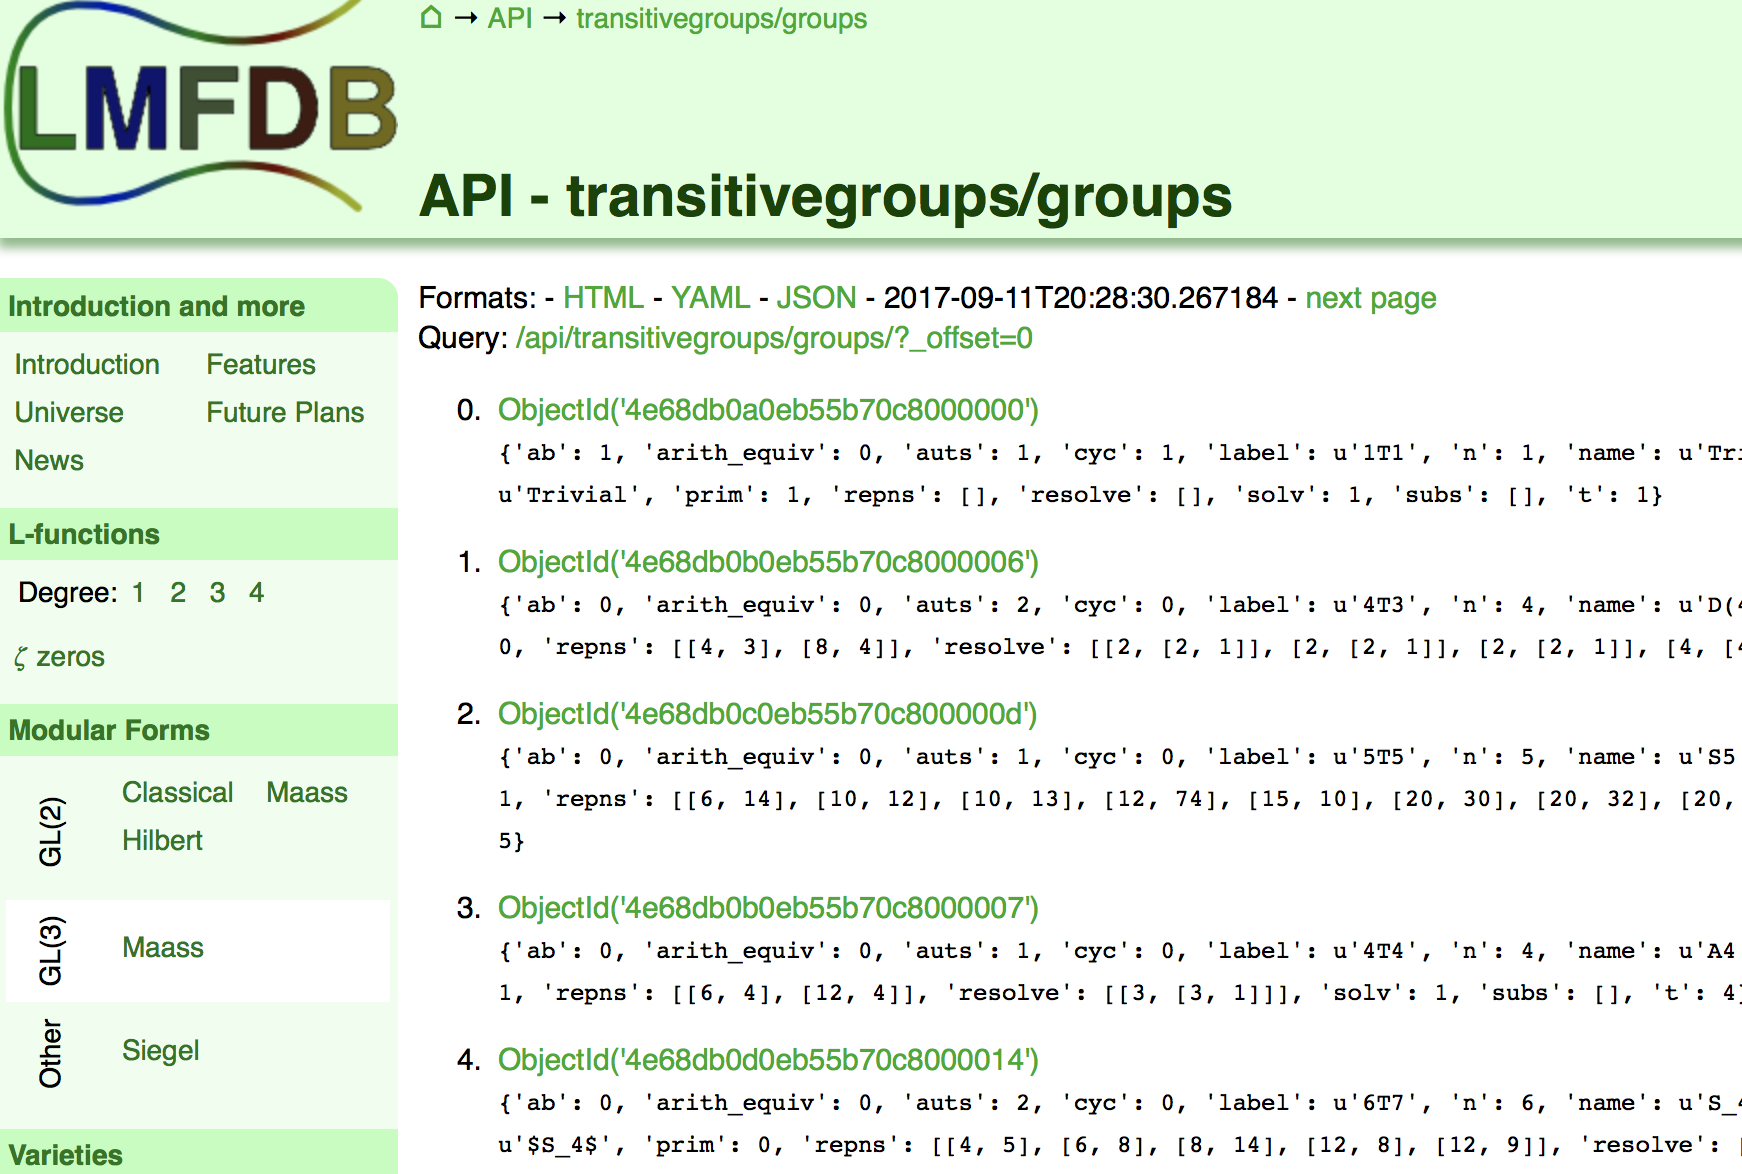
\includegraphics[width=0.7\textwidth]{APIScreenshot}
  \caption[The Web-Interface for the \lmfdb API. ]{
    The Web-Interface for the \lmfdb API. 
  }\vspace*{-1.5em}
  \label{fig:apiscreenshot}
\end{wrapfigure}
Querying is an important application for mathematical knowledge bases.
The \lmfdb API \cite{lmfdbapi} exposes a querying interface that can be used either by humans via the web or programmatically via JSON-based GET requests.
A screenshot of the former interface can be seen in Figure~\ref{fig:apiscreenshot}. 

Queries must name the sub-database to be queried and consist of a set of key-value pairs that correspond to an SQL \texttt{where} clause.
However, while \lmfdb offers a programmable API for accessing its contents, this API sits at the level of the underlying MongoDB, and not the level of mathematical objects. 
For example, to retrieve all Abelian objects in the subdatabase of transitive groups, we expect to use the key-value pair \identifier{commutative}$ = $ \identifier{true}. 
However, these values need to be encoded to be understood by MongoDB.
We need to realize that the database schema actually uses the key \identifier{ab} for commutativity, that it has boolean values, and that the schema encodes \inlinecode{true} as \inlinecode{1}. 
Thus, the actual query to send is \url{http://www.lmfdb.org/api/transitivegroups/groups/?ab=1}. 

In this example, all steps are relatively straightforward. 
But in general, e.g. when searching for all elliptic curves with a specific isogeny matrix, this not only requires good familiarity with the mathematical background but also with the system internals of the particular \lmfdb sub-database; a skill set commonly found in neither research programmers nor average mathematicians.   

Our diagnosis is that {\lmfdb} -- and most other mathematical knowledge databases -- suffer from two problems:
\begin{compactitem}
\item \emph{human/computer mismatch}: humans have problems interacting with \lmfdb because they must speak the system language instead of mathematical language
\item \emph{computer/computer mismatch}: mathematical computer systems cannot interoperate with \lmfdb because their system languages differ.
\end{compactitem}
Using the MitM approach we have presented in Section~\ref{sec:mmtmitm}, we can solve both problems at the same time by lifting the communication to the level of \ommt-encoded MitM objects, which both MitM-compatible software systems and humans can understand.
%%% Local Variables:
%%% mode: latex
%%% TeX-master: "paper"
%%% End:

%  LocalWords:  sec:sota lmfdb lmfdb lstlisting json ainvs iwp0 2adic_gens isogeny_matrix
%  LocalWords:  tamagawa_product 2adic_index anlist 4f71d4304d47869291435e6e vspace emph
%  LocalWords:  fig:lmfdbexample isogeny includegraphics textwidth fig:apiscreenshot
%  LocalWords:  centering summarize sec:mmtmitm ommt-encoded 4f71d4304d47869291435e6e
%  LocalWords:  serialization wrapfigure

 \subsection[Virtual Theories]{\lmfdb as a Set of Virtual Theories}\label{sec:vt}
  % !TEX root = ../thesis.tex
\section{Using Codecs To Implement \lmfdb Virtual Theories}\label{sec:vt}

From a system perspective, virtual theories behave just like concrete theories, but
without the assumption of loading all declarations from a file on disk at system startup.
Instead, virtual theories load declarations in a lazy fashion when they are
needed. Concrete theories are stored as XML files; i.e. we use the file system as a
backend for the \mmt system. As most of the knowledge sources we want to embed into \ommt
as virtual theories use data-bases as back-ends and provide low-level database APIs we
have extended the \mmt backends for this as well. Apart from standard software engineering
tasks, there were three conceptual problems to be solved in this extension/implementation:
\begin{compactenum}[\bf P1]
\item How to match the database tables into \ommt theories and declarations. 
\item How to lift data in \textbf{physical representation} -- i.e. as records of the
  underlying database to \ommt terms -- i.e. data in \textbf{semantic representation}.
\item And how to translate QML queries from semantic to physical representation -- i.e. so
  that they can be executed directly on the data base without loading bulk data into the
  \mmt process.
\end{compactenum}
We will discuss all three using the \lmfdb case discussed above as a running
example. \textbf{P1} can only be solved for each concrete application: Generally, we need
to represent \lmfdb as a set of \ommt theories.  As each sub-database in \lmfdb contains
records of similar structure, it makes sense to create a single virtual theory for each of
these sub-databases and use \ommt declarations for each of the objects. We address
\textbf{P2} next.

\subsection{Translating between Physical and Semantic Representations}\label{sec:vt:translation}

Consider, for example the \identifier{degree} field from the example above.  We have
already seen that this represents the degree of a curve and is an integer value, in this
case the integer $1$.  As \lmfdb uses MongoDB, which is based on JSON, integer values will
usually be represented as a JSON numbers, i.e. an \identifier{IEEE 754} $64$ bit floating
point number.  Here this is the floating point value $1.0$. But when the semantic
representations can exceed the have a maximum possible value $2^{53}-1$ of IEEE floats,
\lmfdb uses a different encoding, e.g. JSON strings that have no hard upper limit.

Let us call the set of objects in semantic representation the \textbf{semantic type}, and
the set of objects in the physical representation the \textbf{realized type}.  Semantic
types reside in the MiTM ontology, whereas realized types resides in the systems
themselves. Corresponding with intuition, the process of converting between the two
representations is called \textbf{coding}, specifically coding into a semantic
representation is called \textbf{encoding}, the reverse is called \textbf{decoding}. We
will call system components that do the necessary translation -- \underline{co}ding and
\underline{dec}oding -- \textbf{CoDec}s. 

As \ommt is a typed framework, we can directly use \ommt types from the MitM ontology for
the semantic types. Simple realized types are usually atomic database types whereas
complex realized types correspond to database tables or views; the details of this setup
are determined by the database schema. To arrive at a tight integration with the \ommt
functionality we will represent as much of this information in \ommt as possible.

Therefore we introduce a new \ommt theory \texttt{Codecs} in the foundational part of the
MitM ontology. See Figure~\ref{fig:vtarch} for details how this plays in the overall
information architecture and Figure~\ref{fig:codecs} for elementary content. This theory
introduces a type constructor \codectt, which given a semantic type constructs the type of
codecs for this type. For instance, the object \identifier{StandardPos} is (a CoDec) of
type $\codectt\;\mathbb{Z}^+$, i.e. a CoDec that parses database objects (for \lmfdb a
IEEE floats) into \ommt terms that can be typed as MitM positive integers and serializes
them back.

\begin{figure}[ht]\centering
  \begin{tikzpicture}\footnotesize
    \node[thy] (codecs) at (0,0) {
      \begin{tabularx}{.84\textwidth}{lll|X}
        \multicolumn{4}{l}{\textsf{Codecs}} \\\hline\hline   
        \identifier{codec}    & : & \multicolumn{1}{l}{$\typett\rightarrow\typett$} & \\\hline
        \identifier{StandardPos}    & : & $\codectt\; \mathbb{Z}^{+}$   & \multirow{3}{*}{\begin{minipage}{3.8in}
                                                                                      JSON number if small enough, \\
                                                                                      else JSON string of decimal expansion
                                                                                      \end{minipage}}\\
        \identifier{StandardNat}    & : & $\codectt\; \mathbb{N}$       & \\
        \identifier{StandardInt}    & : & $\codectt\; \mathbb{Z}$       & \\\hline
        \identifier{IntAsArray}     & : & $\codectt\; \mathbb{Z}$       & JSON List of Numbers\\
        \identifier{IntAsString}    & : & $\codectt\; \mathbb{Z}$       & JSON String of decimal expansion\\\hline
        \identifier{StandardBool}   & : & $\codectt\; \mathbb{B}$       & JSON Booleans \\
        \identifier{BoolAsInt}      & : & $\codectt\; \mathbb{B}$       & JSON Numbers $0$ or $1$ \\\hline
        \identifier{StandardString} & : & $\codectt\; \mathbb{S}$       & JSON Strings \\
      \end{tabularx}
    };
  \end{tikzpicture}
  \caption[List of Codecs]{
    An annotated subset of the Codecs theory containing a selection of codecs found in \mmt. 
    Here $\mathbb{N}$ represents natural numbers (including $0$), 
    $\mathbb{Z}$ integers, 
    $\mathbb{Z}^{+}$ positive integers, 
    $\mathbb{B}$ booleans and
    $\mathbb{S}$ (unicode character) strings. 
  }
  \label{fig:codecs}
\end{figure}
The \identifier{degree} we used as an example above would use the \identifier{StandardInt}
codec. Additionally the \textsf{CoDecs} theory associates with each codec a Scala class
that implements the translation between semantic and realized type.

But codecs for basic types (semantic and realized) is not sufficient for our application.
Consider for example the \identifier{isogeny\_matrix} field of an elliptic curve
representation.  The semantic representation of the value of this field is the matrix
\[M = \left(
    \begin{array}{ccc}
      1 & 5 & 25 \\
      5 & 1 & 5 \\
      25 & 5 & 1 \end{array} 
  \right)
\]
Matrices are characterized with three parameters, the type of object they contain
(integers in this case) along their row and column count ($3 \times 3$ in this case).  In
principle, one could construct a codec for each type of matrices by hand.  This would mean
generating one codec for $1 \times 1$ integer matrices, $1 \times 1$ real matrices,
$1 \times 2$ integer matrices, $1 \times 2$ real matrices, and so on.  For the
representation of codecs in \mmt, this would require generating one symbol and one Scala
function for each different kind of matrix.  This quickly becomes a mess.

Instead we use the fact that both Scala and \ommt allow higher-order functions: We can
define a \textbf{codec operator} that given a codec the parameter type $\tau$ and values
for the number $n$ of rows and $m$ of columns, generate a codec of $n\times m$ matrices of
$\tau$ objects. In the example above and the matrix $M$ is encoded as a list of $n$ lists
of $m$ integers ($\tau$):
% HACK HACK HACK overfull box\\\noindent
\inlinecode{[[1.0,5.0,25.0],[5.0,1.0,5.0],[25.0,5.0,1.0]]}

\begin{figure}[ht]\centering
  \begin{tikzpicture}\footnotesize
    \node[thy] (codecs) at (0,0) {
      \begin{tabularx}{\textwidth}{lll|X}
        \multicolumn{4}{l}{\textsf{Codecs (continued)}} \\\hline\hline   
        \identifier{StandardList}    & : & 
                 $\left\{T\right\} \codectt\; T \rightarrow \codectt\; \mathrm{List}(T)$ & 
                  JSON list, recursively coding each element of the list\\\hline
        \identifier{StandardVector}    & : & 
                  $\left\{T, n\right\} \codectt\; T \rightarrow \codectt\; \mathrm{Vector}(n, T)$ & 
                   JSON list of fixed length $n$\\\hline
        \identifier{StandardMatrix}    & : & 
                   $\left\{T, n, m\right\} \codectt\; T \rightarrow \codectt\; \mathrm{Matrix}(n, m, T)$ & 
                   JSON list of $n$ lists of length $m$\\
      \end{tabularx}
    };
  \end{tikzpicture}
  \caption[List of Codec Operators]{
    Second annotated subset of the codecs theory containing a selection of codec operators found in \mmt. 
    Compare with Figure~\ref{fig:codecs}. 
  }
  \label{fig:codecops}
\end{figure}
Like first-order codecs, codec operators in \mmt are again represented in two ways, as
declarations inside the \identifier{CoDecs} theory (see Figure~\ref{fig:codecops} for a
list) and as a corresponding Scala implementation -- a higher-order function from CoDecs
to CoDecs. This is mirrored in the types of operators in Figure~\ref{fig:codecs}: the
\textsf{StandardMatrix} operator is a function that takes four arguments: a type $T$, two
numbers $n$ and $m$, and a $\tau$-codec and yields a $\mathrm{Matrix}(n, m,
T)$-codec. Here we make use of the dependent function types of the MitM foundation:
arguments in curly brackets can be used in the result type; see~\cite{RabKoh:WSMSML13} for
details.

With these declarations in the \textsf{CoDecs} theory, we can represent a codec for
$3 \times 3$ integer matrices e.g. for the the isogeny matrix $M$ above by the \ommt term
$\plaintt{StandardMatrix}(3, 3, \plaintt{StandardInt})$\footnote{The observant reader will
  have noticed that the way codec operators have been declared, the codec in question
  actually corresponds to the term
  $\plaintt{StandardMatrix}(\mathbb{Z}, 3, 3, \plaintt{StandardInt})$.  This has an
  additional $\mathbb{Z}$ as the first argument.  However, the last argument is a codec
  for a specific semantic type and thus fully determines the first argument.  \mmt is
  capable of transparently inferring the first argument, thus it can be omitted for
  readability without needing any kind of special treatment implementation wise.  }.
Similarly the same codec operator can be used to for example generate a codec for
$2 \times 2$ boolean matrices, which corresponds to
$\plaintt{StandardMatrix}(2, 2, \plaintt{StandardBool})$.

\subsection{Schema Information in Virtual Theories}\label{sec:vt:schemas}

\begin{figure}[ht]\centering
    \begingroup
    \pgfdeclarelayer{background}
    \pgfdeclarelayer{foreground}
    \pgfsetlayers{background,foreground}
    
    \resizebox{\textwidth}{0.75\textwidth}{
      \begin{tikzpicture}[xscale=4,yscale=3]\footnotesize
        \begin{pgfonlayer}{foreground}
          \tikzstyle{human}    = [red,dashed,thick]
          \tikzstyle{withshadow}  = [draw,drop shadow={opacity=.5},fill=white]
          \tikzstyle{interface}   = [fill=blue!30]
          \tikzstyle{database}    = [cylinder,cylinder uses custom fill,
            cylinder body fill=yellow!50,cylinder end fill=yellow!50,
            shape border rotate=90,
            aspect=0.25,draw]
          
          % Ontology layer
          \node[thy] (numbers) at (0,1) {
            \begin{tabular}{lll}
              \multicolumn{3}{l}{\textsf{Numbers}}\\\hline\hline
              $\mathbb{Z}^{+}$        & : & \typett\\
              $\mathbb{Z}$            & : & \typett\\\hline
              \multicolumn{3}{l}{$\mathbb{Z}^{+} \subset \mathbb{Z}$}
            \end{tabular}
          };

          \node[thy] (matrices) at (1.5,1) {
            \begin{tabular}{lll}
              \multicolumn{3}{l}{\textsf{Matrices}}\\\hline\hline
              \plaintt{matrix} & : & $\typett \rightarrow \mathbb{Z}^{+}\rightarrow \mathbb{Z}^{+} \rightarrow \typett$
            \end{tabular}
          };

          \node[thy] (codecs) at (0.75,0) {
            \begin{tabular}{lll}
              \multicolumn{3}{l}{\textsf{Codecs}}\\\hline\hline
              \codectt                  & : & $\typett \rightarrow \typett$\\\hline
              \plaintt{standardInt}     & : & $\codectt\; \mathbb{Z}$\\
              \plaintt{standardMatrix}  & : & $\left\{T, n, m\right\} \codectt\; T \rightarrow \codectt\; \plaintt{matrix}(n, m, T)$\\
            \end{tabular}
          };

          \draw[include] (numbers) -- (matrices);
          \draw[include] (matrices) -- (codecs);
          
          \begin{pgfonlayer}{background}
            \node[draw=none,fill=green!30,rounded corners=1cm,fit=(numbers) (matrices) (codecs),inner sep=15pt] {};
          \end{pgfonlayer}
        
          % Model Layer
          \node[thy] (ec) at (2.25,-1.20) {
            \begin{tabular}{lll}
              \multicolumn{3}{l}{\textsf{Elliptic Curve}}\\\hline\hline
              \plaintt{ec}            & : & \typett\\\hline
              \plaintt{from\_record}  & : & $\plaintt{record} \rightarrow \plaintt{ec}$ \\\hline
              \plaintt{curveDegree}   & : & $\plaintt{ec} \rightarrow \mathbb{Z}$ \\
              \plaintt{isogenyMatrix} & : & $\plaintt{ec} \rightarrow \plaintt{matrix}(3, 3, \mathbb{Z})$ 
            \end{tabular}
          };

          \node[thy,interface] (ecschema) at (2.0,-2.5) {
            \begin{tabular}{lll}
              \multicolumn{3}{l}{\textsf{Elliptic Curve Schema}}\\\hline\hline
              $\plaintt{degree}$            & \uri{?implements}  & \plaintt{curveDegree} \\
                                            & \uri{?codec}       & \plaintt{StandardInt} \\\hline
              $\plaintt{isogeny\_matrix}$   & \uri{?implements}  & \plaintt{isogenyMatrix} \\
                                            & \uri{?codec}       & $\plaintt{StandardMatrix}(3, 3, \plaintt{StandardInt})$ 
            \end{tabular}
          };
          
          \begin{pgfonlayer}{background}
            \node[draw,cloud,fit=(ec),aspect=4,withshadow,inner sep=-4pt,purple!30] {};
          \end{pgfonlayer}

          % Database Layer
          \node[database] (mongodb) at (-.5,-2.5) {
            \textsf{\lmfdb Elliptic Curves}
          };

          \node[thy,interface] (dbtheory) at (0,-1.20) {
            \begin{tabular}{lllll}
              \multicolumn{5}{l}{\textsf{Elliptic Curve Database Theory}}\\\hline\hline
              \plaintt{11a1} & : & $\plaintt{ec}$ & $=$ & \dots\\
              \plaintt{11a2} & : & $\plaintt{ec}$ & $=$ & \dots\\
              \dots
            \end{tabular}
          };
          \draw[include] (matrices.south)+(.75,0) -- (ec.north);
          \draw[include] (ec) -- (dbtheory);
          
          \draw[human,->] (dbtheory) -- node[right]{\scriptsize {lazily loads from}} (mongodb);
          \draw[human,->] (ecschema) -- node[right]{\scriptsize {implements}} (ec);
          \draw[human,->] (ecschema) -- node[above]{\scriptsize {describes}} (mongodb);
        \end{pgfonlayer}
      \end{tikzpicture}
    }
    \endgroup
  \caption[Virtual Theory Architecture]{
    A sketch of the architecture for a virtual theory connecting to \lmfdb. 
    Solid edges represent imports. 
    Several declarations have been omitted for simplicity. 
  }
  \label{fig:vtarch}
\end{figure}

Codecs enable creation of individual values within \lmfdb and mathematical databases in general. 
This is not enough -- a mechanism to translate entire records as a whole is needed to implement a Virtual Theory. 

The architecture of a virtual theory for \lmfdb elliptic curves is illustrated in Figure~\ref{fig:vtarch}. 
It consists of four different parts, the foundational ontology theories (colored in green), mathematical model ontology (colored in red), database interface theories (colored in blue) and \lmfdb itself (colored in yellow). 
These aspects originate from the Math-In-The-Middle approach. 

The foundational ontology theories provide a system-independent basis for the remainder of the approach. 
In this example, they first define a type of integers $\mathbb{Z}$ and positive integers $\mathbb{Z}^{+}$ and then proceed to define a \identifier{matrix} type. 
This type takes three parameters, a type of elements in the matrix, and then a row and column count. 
Next, the codec \identifier{standardInt} and codec operator \identifier{standardMatrix} are defined as previously. 

Next, the \textit{Elliptic Curve} theory is described. 
It models an elliptic curve in a very simple fashion, by just declaring a type \identifier{ec}. 
Next, it defines a \identifier{from\_record} constructor that takes an \mmt record and returns an elliptic curve. 
Notice that these definitions are independent of the \lmfdb database. 

The theory then moves on to define the two important properties\footnote{In reality there
  are of course more than these two -- the others can be implemented analogously and are
  omitted here to better illustrate this example.} of elliptic curves.  These are
\textit{degree}, an integer, and the \textit{isogeny matrix}, a $3 \times 3$ matrix of
integers. They are modeled as functions that take an elliptic curve and return the
appropriate type.  Recall that the Math-In-The-Middle approach aims to model mathematical
knowledge ``in the middle'' independent of any particular system.  This is exactly the
case here -- the model of elliptic curves does not rely on \lmfdb, nor any other system,
so that we can integrate other knowledge sources about elliptic curves or to future
versions of the \lmfdb with changed struture.

\subsection{Knowledge Source Integration in MitM}

Given this infrastructure, let us see how we can integrate knowledge sources like the
\lmfdb in the Math-In-The-Middle approach. Instead of the API CDs presented in
Section~\ref{sec:mmtmitm}, we use an integrated approach that is based on \textbf{schema
  theory} that internalizes the \lmfdb schema and the \textbf{database theory}, a virtual
theory that represents the \lmfdb data.

The schema theory, as the name suggests, describes the schema of the \lmfdb elliptic curve
database.  This is the only place in the entire architecture of virtual theories which
relies on the structure of \lmfdb.  The schema theory contains declarations for each field
within an \lmfdb record.  The name of these declarations corresponds to the name of the
field inside the record.  Each declaration is annotated using \mmt meta-data with two
pieces of information, the property of an elliptic curve it implements and the codec that
is used to encode it inside \lmfdb.  For example, the \identifier{degree} field implements
the \identifier{curveDegree} property in the elliptic curve theory and uses the
\identifier{StandardInt} codec.

The other is the database theory. This is the truly virtual theory -- it is not stored on
disk, but generated dynamically.  As designed, it contains one declaration per record in
\lmfdb. It uses an \mmt \textbf{backend} -- an \mmt abstraction used to load declarations
into memory.  Given a URI, the backend is responsible for loading the underlying
definition.  For the elliptic curve theories these URIs are of the form
\uri{lmfdb:db/transitivegroups?groups?11A1}.\ednote{MK@TW: really transitive groups?}

The backend first retrieves the appropriate record from {\lmfdb} -- in the case of
\identifier{11A1} this corresponds to retrieving the JSON found in
Figure~\ref{fig:lmfdbexample}.  Next, the backend attempts to turn this JSON into an \mmt
record so that it can be passed to the \identifier{from\_record} constructor.

For this, it needs all declarations in the schema theory.  Each of these declarations
corresponds to a single field in the JSON, that can be turned into a field of the \mmt
record.  In the example provided here, we only consider two fields, \identifier{degree}
and \identifier{isogeny_matrix}.

For each of these two fields, the backend knows which field to create in the \mmt record
that it has to construct.  They are given by the \identifier{?implements} meta-datum, here
\identifier{curveDegree} and \identifier{isogenyMatrix}.  But this information is not
enough.  The JSON values of the fields can not be used as values inside an \mmt record,
they need to be assigned their correct semantics first.

This is where codecs and the \identifier{?codec} meta-datum come into play. 
The physical representation of the \identifier{degree} field is $1$, a JSON integer. 
The schema theory says that this is encoded using the \identifier{StandardInt} codec from above. 
To generate an \mmt value for the record, this codec can be used to decode it. 
In this case the decoded value is the integer $1$\footnote{
  In this document, the physical and semantic representation are rendered in the same fashion. 
  It is important to realize that they are not in fact the same. 
  The physical representation is a 64-bit floating point JSON Number $1$, whereas the semantic representation is the integer $1$. 
  Technically, the semantic representation is actually the \ommt integer literal $1$. 
  We skim over this detail here, as the \ommt literals are designed to precisely represent this value. 
}. 

The physical representation of \identifier{isogenyMatrix} is
\inlinecode{[[1.0,5.0,25.0],[5.0,1.0,5.0],[25.0,5.0,1.0]]}.  Here, the schema theory
contains a codec that is constructed using the \identifier{StandardMatrix} codec operator,
specifically \\$\plaintt{StandardMatrix}(3, 3,
\plaintt{StandardInt})$.  To apply this codec, the Backend has to first construct the
concrete codec, which can then used to decode the physical representation.  Since this is
a codec operator, first each entry of the matrix has to be decoded using
$\plaintt{StandardInt}$ -- turning the JSON number $1.0$ into the integer
$1$, the JSON Number $5.0$ into the number
$5$, etc.  Then these decoded values can be placed inside a matrix to arrive at the
semantic representation\footnote{Similar to the semantic representation above, the matrix
  $M$ is technically different from the \ommt representation.  We could again represent
  this using a matrix literal, but instead the implementation actually uses a constructor
  containing integer literals.  For simplicity, and as literals are designed to precisely
  represent mathematical objects, we omit this detail.  } 
\[M = \left( \begin{array}{ccc}
               1 & 5 & 25 \\
               5 & 1 & 5 \\
               25 & 5 & 1 
             \end{array}
           \right)
\]

This gives the backend all the information it needs to construct an \mmt record which can
then be turned into an elliptic curve using the \identifier{from\_record} constructor.
The \identifier{degree} field is assigned the value
$1$ and the \identifier{isogenyMatrix} is assigned the value of the matrix $M$.  Finally,
this \mmt term can be used to define a new constant inside the database theory.

%%% Local Variables:
%%% mode: latex
%%% TeX-master: "paper"
%%% End:

%  LocalWords:  sec:vt lmfdb ommt textit textit realized tikzpicture tabularx textwidth
%  LocalWords:  hline hline rightarrow codectt mathbb multirow fig:codecs isogeny mathrm
%  LocalWords:  characterized noindent formalized fig:codecops plaintt plaintt begingroup
%  LocalWords:  pgfdeclarelayer pgfsetlayers background,foreground resizebox xscale ec
%  LocalWords:  4,yscale pgfonlayer tikzstyle red,dashed,thick withshadow draw,drop oding
%  LocalWords:  cylinder,cylinder 50,cylinder 0.25,draw none,fill 30,rounded 1cm,fit
%  LocalWords:  thy,interface ecschema draw,cloud,fit 4,withshadow,inner 4pt,purple
%  LocalWords:  mongodb dbtheory endgroup fig:vtarch colored colored colored colored
%  LocalWords:  fig:lmfdbexample textbf centering RabKoh:WSMSML13 sec:mmtmitm
%  LocalWords:  internalizes

 \subsection{Ascribing Encodings in Schema Theories}\label{sec:vt:codec}
  % !TEX root = ../thesis.tex
\section{Accessing Virtual Theories}\label{sec:access}

We address \textbf{P2} next.
Intuitively, it is straightforward how to fill a virtual theory $V$: $V$ is represented by an initially empty concrete theory $V'$, and whenever an identifier $id$ of $V$ is requested, \mmt dynamically adds the corresponding declaration of $id$ to $V'$.
\mmt already abstracts from the physical realizations of persistent storage using the \emph{backend} interface: essentially a backend is any component that allows loading declarations.
Thus, we only have to implement a new backend that connects to \lmfdb, retrieves the JSON object with identifier $id$, and turns into an \ommt declaration.

However, this glosses over a major problem: the databases used for the physical storage of large datasets usually relatively simple data structure.
For example, a JSON database (as underlies \lmfdb) offers only limited-precision integers, boolean, strings, lists, and records as primitive objects and does not provide a type system.
Consequently, the objects stored in the database are very different from the sophisticated mathematical objects expected by the schema theory.
Therefore, databases like \lmfdb must encode this complex mathematical objects as simple database objects.

\subsection{Concrete Encodings of Mathematical Objects}\label{sec:vt:translation}

Consider, for example the \identifier{degree} field from Figure~\ref{fig:lmfdbexample} above. 
It's value is the integer $1$, representing the degree of this curve. 
However inside the database it is represented as the \identifier{IEEE 754} $64$-bit floating point number $1.0$. 
But when the semantic representations can exceed the have a maximum possible value $2^{53}-1$ of IEEE floats, \lmfdb needs to use a different encoding, e.g. JSON strings that have no hard upper limit.

Let us call the set of objects in semantic representation the \textbf{semantic type}, and the set of objects in the physical representation the \textbf{realized type}. 
Semantic types reside in the MiTM ontology, whereas realized types describe structures of the systems themselves -- here the tables in the \lmfdb. 
Corresponding with intuition, the process of converting between the two representations is called \textbf{coding}, specifically coding into a semantic representation is called \textbf{encoding}, the reverse is called \textbf{decoding}. 
We will call system components that do the necessary translation -- \underline{co}ding and \underline{dec}oding -- \textbf{CoDec}s. 

As \ommt is a typed framework, we can directly use \ommt types from the MitM ontology for the semantic types. 
Simple realized types are usually atomic database types whereas complex realized types correspond to database tables or views; the details of this setup are determined by the database schema. 
To arrive at a tight integration with the \ommt functionality we will represent as much of this information in \ommt as possible.

Therefore we introduce a new \ommt theory \texttt{Codecs} in the foundational part of the MitM ontology.  
See the green part of Figure~\ref{fig:vtarch} for details how this plays in the overall information architecture and Figure~\ref{fig:codecs} for elementary content. 
This theory introduces a type constructor \codectt, which given a semantic type constructs the type of CoDecs for this type. 
For instance, the object \identifier{StandardPos} is (a CoDec) of type $\codectt\;\mathbb{Z}^+$, i.e. a CoDec that parses database objects (for \lmfdb IEEE floats) into \ommt terms that can be typed as MitM positive integers and serializes them back.

\begin{figure}[ht]\centering
  \begin{tikzpicture}\footnotesize
    \node[thy] (codecs) at (0,0) {
      \begin{tabularx}{.84\textwidth}{lll|X}
        \multicolumn{4}{l}{\textsf{Codecs}} \\\hline\hline   
        \identifier{codec}    & : & \multicolumn{1}{l}{$\typett\rightarrow\typett$} & \\\hline
        \identifier{StandardPos}    & : & $\codectt\; \mathbb{Z}^{+}$   & \multirow{3}{*}{\begin{minipage}{3.8in}
                                                                                      JSON number if small enough, \\
                                                                                      else JSON string of decimal expansion
                                                                                      \end{minipage}}\\
        \identifier{StandardNat}    & : & $\codectt\; \mathbb{N}$       & \\
        \identifier{StandardInt}    & : & $\codectt\; \mathbb{Z}$       & \\\hline
        \identifier{IntAsArray}     & : & $\codectt\; \mathbb{Z}$       & JSON List of Numbers\\
        \identifier{IntAsString}    & : & $\codectt\; \mathbb{Z}$       & JSON String of decimal expansion\\\hline
        \identifier{StandardBool}   & : & $\codectt\; \mathbb{B}$       & JSON Booleans \\
        \identifier{BoolAsInt}      & : & $\codectt\; \mathbb{B}$       & JSON Numbers $0$ or $1$ \\\hline
        \identifier{StandardString} & : & $\codectt\; \mathbb{S}$       & JSON Strings \\
      \end{tabularx}
    };
  \end{tikzpicture}
  \caption[List of Codecs]{
    An annotated subset of the Codecs theory containing a selection of CoDecs found in \mmt. 
    Here $\mathbb{N}$ represents natural numbers (including $0$), 
    $\mathbb{Z}$ integers, 
    $\mathbb{Z}^{+}$ positive integers, 
    $\mathbb{B}$ booleans and
    $\mathbb{S}$ (unicode character) strings. 
  }
  \label{fig:codecs}
\end{figure}
The \identifier{degree} we used as an example above would use the \identifier{StandardInt} CoDec in the \lmfdb. 
Additionally the \textsf{CoDecs} theory associates with each CoDec a Scala class that implements the translation between semantic and realized type. The \mmt system we use is implemented in Scala and can thus execute this class as part of \lmfdb access. 

\begin{wrapfigure}r{2.7cm}\vspace*{-2em}
$M = \left(
    \begin{array}{ccc}
      1 & 5 & 25 \\
      5 & 1 & 5 \\
      25 & 5 & 1 \end{array} 
  \right)$\vspace*{-1em}
\end{wrapfigure}
But CoDecs for basic types (semantic and realized) are not sufficient for our application.
Consider again the \identifier{11a1} curve shown in Figure~\ref{fig:lmfdbexample}, specifically the \identifier{isogeny\_matrix} field. 
The semantic representation of the value of this field is the matrix on the right.

The semantic type of Matrices is characterized with three parameters, the type of object they contain (integers in this case) along their row and column count ($3 \times 3$ in this case). 
In principle, one could construct a CoDec for each type of matrices by hand. 
This would mean generating one CoDec for $1 \times 1$ integer matrices, $1 \times 1$ real matrices, $1 \times 2$ integer matrices, $1 \times 2$ real matrices, and so on. 
For the representation of CoDecs in \mmt, this would require generating one symbol and one Scala function for each different kind of matrix. 
This quickly becomes a mess.

Instead we use the fact that both Scala and \ommt allow higher-order functions: 
We can define a \textbf{CoDec operator} that -- given a CoDec, the parameter type $\tau$, and values for the number $n$ of rows and $m$ of columns --  generates a CoDec for $n\times m$ matrices of $\tau$ objects. 
In the example above and the matrix $M$ is encoded as a list of $n$ lists of $m$ integers ($\tau$):
\begin{lstlisting}[]
[[1.0,5.0,25.0],[5.0,1.0,5.0],[25.0,5.0,1.0]]
\end{lstlisting}

\begin{figure}[ht]\centering
  \begin{tikzpicture}\footnotesize
    \node[thy] (codecs) at (0,0) {
      \begin{tabularx}{\textwidth}{lll|X}
        \multicolumn{4}{l}{\textsf{Codecs (continued)}} \\\hline\hline   
        \identifier{StandardList}    & : & 
                 $\left\{T\right\} \codectt\; T \rightarrow \codectt\; \mathrm{List}(T)$ & 
                  JSON list, recursively coding each element of the list\\\hline
        \identifier{StandardVector}    & : & 
                  $\left\{T, n\right\} \codectt\; T \rightarrow \codectt\; \mathrm{Vector}(n, T)$ & 
                   JSON list of fixed length $n$\\\hline
        \identifier{StandardMatrix}    & : & 
                   $\left\{T, n, m\right\} \codectt\; T \rightarrow \codectt\; \mathrm{Matrix}(n, m, T)$ & 
                   JSON list of $n$ lists of length $m$\\
      \end{tabularx}
    };
  \end{tikzpicture}
  \caption[List of Codec Operators]{
    Second annotated subset of the CoDecs theory containing a selection of CoDec operators found in \mmt. 
    Compare with Figure~\ref{fig:codecs}. 
  }
  \label{fig:codecops}
\end{figure}
Like first-order CoDecs, CoDec operators in \mmt are again represented in two ways, as declarations inside the \identifier{CoDecs} theory (see Figure~\ref{fig:codecops} for a list, also compare again with Figure~\ref{fig:vtarch}) and as a corresponding Scala implementation -- a higher-order function from CoDecs to CoDecs. 
This is mirrored in the types of operators in Figure~\ref{fig:codecs}, the \textsf{StandardMatrix} operator is a function that takes four arguments: a type $T$, two
numbers $n$ and $m$, and a $\tau$-CoDec and yields a $\mathrm{Matrix}(n, m, T)$-CoDec. 
Here we make use of the dependent function types of the MitM foundation: arguments in curly brackets can be used in the result type; see~\cite{RabKoh:WSMSML13} for details.

With these declarations in the \textsf{CoDecs} theory, we can represent a CoDec for $3 \times 3$ integer matrices e.g. for the the isogeny matrix $M$ above by the \ommt term $\plaintt{StandardMatrix}(3, 3, \plaintt{StandardInt})$.
Similarly the same CoDec operator can be used to for example generate a CoDec for $2 \times 2$ boolean matrices, which corresponds to
$\plaintt{StandardMatrix}(2, 2, \plaintt{StandardBool})$. 

\subsection{Specifying Encodings in Schema Theories}

Given this infrastructure, let us see how we can integrate knowledge sources like the \lmfdb in the Math-In-The-Middle approach. 
The schema theory, as the name suggests, describes the schema of the \lmfdb elliptic curve database. 
This is the only place in the entire architecture of virtual theories which relies on the structure of \lmfdb. 
The schema theory contains declarations for each field within an \lmfdb record. 
The name of these declarations corresponds to the name of the field inside the record. 
Each declaration is annotated using \mmt meta-data with two pieces of information, the property of an elliptic curve it implements and the codec that is used to encode it inside \lmfdb. 
For example, the \identifier{degree} field implements the \identifier{curveDegree} property in the elliptic curve theory and uses the \identifier{StandardInt} codec.

The database theory is the only truly virtual theory -- it is not stored on disk, but generated dynamically. 
It can again be seen in Figure~\ref{fig:vtarch}. 
As designed, it contains one declaration per record in \lmfdb. 
It uses an \mmt \textbf{backend} -- an \mmt abstraction used to load declarations into memory. 
Given a URI, the backend is responsible for loading the underlying definition. 
For the elliptic curve theories these URIs are of the form \uri{lmfdb:db/elliptic_curves?curves?11A1}. 

The backend first retrieves the appropriate record from {\lmfdb} -- in the case of \identifier{11A1} this corresponds to retrieving the JSON found in Figure~\ref{fig:lmfdbexample}. 
Next, the backend attempts to turn this JSON into an \mmt record so that it can be passed to the \identifier{from\_record} constructor.

For this, it needs all declarations in the schema theory. 
Each of these declarations corresponds to a single field in the JSON, that can be turned into a field of the \mmt record. 
In the example provided here, we only consider two fields, \identifier{degree} and \identifier{isogeny_matrix}.

For each of these two fields, the backend knows which field to create in the \mmt record that it has to construct. 
They are given by the \identifier{?implements} meta-datum, here \identifier{curveDegree} and \identifier{isogenyMatrix}. 
But this information is not enough. 
The JSON values of the fields can not be used as values inside an \mmt record, they need to be assigned their correct semantics first.

This is where CoDecs and the \identifier{?codec} meta-datum come into play. 
The physical representation of the \identifier{degree} field is $1$, a JSON integer. 
The schema theory says that this is encoded using the \identifier{StandardInt} CoDecs from above. 
To generate an \mmt value for the record, this codec can be used to decode it. 
In this case the decoded value is the integer $1$. 
Notice how even though the physical and semantic representations are shown identically here, they are indeed different: The former is a 64-bit floating point JSON Number, the latter is a mathematical integer. 

The physical representation of \identifier{isogenyMatrix} is
% HACK HACK HACK -- TeX can't do proper line breaking
\\\noindent\inlinecode{[[1.0,5.0,25.0],[5.0,1.0,5.0],[25.0,5.0,1.0]]}. 
Here, the schema theory contains a CoDecs that is constructed using the \identifier{StandardMatrix} codec operator, specifically $\plaintt{StandardMatrix}(3, 3, \plaintt{StandardInt})$. 
To apply this CoDecs, the backend has to first construct the concrete CoDecs, which can then used to decode the physical representation. 
Since this is a CoDecs operator, first each entry of the matrix has to be decoded using $\plaintt{StandardInt}$ -- turning the JSON number $1.0$ into the integer $1$, the JSON Number $5.0$ into the number $5$, etc. 
Then these decoded values can be placed inside a matrix to arrive at the semantic representation of $M$. 

This gives the backend all the information it needs to construct an \mmt record which can then be turned into an elliptic curve using the \identifier{from\_record} constructor. 
The \identifier{degree} field is assigned the value $1$ and the \identifier{isogenyMatrix} is assigned the value of the matrix $M$. 
Finally, this \mmt term can be used to define a new constant inside the database theory.


%%% Local Variables:
%%% mode: latex
%%% TeX-master: "paper"
%%% End:

%  LocalWords:  sec:vt lmfdb ommt textit textit realized tikzpicture tabularx textwidth
%  LocalWords:  hline hline rightarrow codectt mathbb multirow fig:codecs isogeny mathrm
%  LocalWords:  characterized noindent formalized fig:codecops plaintt plaintt begingroup
%  LocalWords:  pgfdeclarelayer pgfsetlayers background,foreground resizebox xscale ec
%  LocalWords:  4,yscale pgfonlayer tikzstyle red,dashed,thick withshadow draw,drop oding
%  LocalWords:  cylinder,cylinder 50,cylinder 0.25,draw none,fill 30,rounded 1cm,fit
%  LocalWords:  thy,interface ecschema draw,cloud,fit 4,withshadow,inner 4pt,purple
%  LocalWords:  mongodb dbtheory endgroup fig:vtarch colored colored colored colored
%  LocalWords:  fig:lmfdbexample textbf centering RabKoh:WSMSML13 sec:mmtmitm
%  LocalWords:  internalizes

 \subsection{Translating Queries}\label{sec:qmt}
  % !TEX root = ../thesis.tex
Recall that \mmt has a general-purpose Query Language called QMT~\cite{Rabe:qlfml12}, which allows users to find knowledge subject to even complex conditions. 
We continue by briefly addressing \textbf{P3}: query translation; for a complete discussion we refer the interested reader to \cite{twiesing:msc17}. 

In practice, most queries involving virtual theories so far have a shape similar to the one that \lmfdb supports: 
Finding all objects within a single sub-database for which a specific field has a specific value. 
As an example, consider again the query of finding all Abelian transitive groups. 
QMT has an \mmt-powered surface syntax, which can be used to express this query as:
\begin{lstlisting}[language=qmt,basicstyle=\small\sf]
x in (related to ( literal `lmfdb:db/transitivegroups?group ) by (object declares)) 
  | holds x (x commutative x *=* true)
\end{lstlisting}

The example consists of two parts, first we find all objects declared in the \uri{lmfdb:db/transitivegroups?group} theory (line 1), and then we restrict this set of results to all those for which the \inlinecode{commutative} property is \inlinecode{true} (line 2). 
Notice that this the example shown here is the formal equivalent of the \lmfdb query shown in Section~\ref{sec:lmfdb}. 
The key difference is that this query does not require knowing the record structure of \lmfdb --
apart from knowing the proper sub-db, instead it only relies on knowing the mathematical
semantics (commutativity) of the query in question. 

Recall that to evaluate a query prior to the introduction of virtual theories, the \mmt system loaded the theory graph into main memory and then interleaved incremental flattening and query evaluation operations on the \mmt data structures until a result had been produced. 
But it is infeasible to first load all potentially relevant data into memory, and only then proceed with evaluation. 
This would require loading a copy of \lmfdb into main memory, something that virtual theories were designed to avoid. 

The low-level API of  \lmfdb and similar system provides a new approach for making queries towards virtual theories. 
First, the \mmt query is translated into a system-specific information-retrieval language --- in the case of \lmfdb\ this is currently a MongoDB-based syntax.
Next, this translated query is sent to the external API. 
Upon receiving the results, these are translated back into \ommt with the help of already existing functionality in the appropriate virtual theory backend.

This leaves just one problem unsolved --- translating queries into the system-specific API. 
However, it is insufficient to simply translate queries as a whole: 
One hand a general QMT query may or may not involve a virtual theory, on the other hand, it may also involve several (unrelated) virtual theories. 
This makes it necessary to filter out queries involving virtual theories, and assign them to a specific backend, and then translate only these parts. 

Achieving this automatically is a non-trivial problem. 
Queries are inductive in nature, and one could attempt to intercept each of the intermediate results. 
However, this would require a check on each intermediate result to first determine if it comes from a virtual theory or not, and then potentially switching the entire evaluation strategy, leading to a computationally expensive implementation. 

Instead of intercepting each result, we extended the Query Language to allow users to annotate sub-queries for evaluation with a specific virtual theory backend. 
This allows the system to immediately know which parts of a query have to be evaluated in \mmt memory, and which have to be translated and sent to an external system. 
This turns the example above into:
\begin{lstlisting}[language=qmt]
use "lmfdb" for {*
  x in (related to ( literal `lmfdb:db/transitivegroups?group ) 
    by (object declares)) | holds x (x commutative x *=* true)
*}
\end{lstlisting}
Here, we have simply wrapped the entire query with a \inlinecode{use lmfdb} statement, indicating the query should be evaluated using \lmfdb. 

The encoding of this specific query can be achieved using codecs.
The query corresponds to the URL \url{http://www.lmfdb.org/api/transitivegroups/groups/?ab=1}. 
Next, the \lmfdb API returns a set of JSON objects corresponding to all Abelian transitive groups. 
These can then be decoded into \ommt objects using the procedure described in Section~\ref{sec:vt:codec}, i.e. for each field we look up the corresponding codec and use it to deconstruct the field, eventually creating an \mmt record. 
Afterwards, these \ommt terms can then be passed to the user as a result to the query. 
%%% Local Variables:
%%% mode: latex
%%% TeX-master: "report"
%%% End:

%  LocalWords:  sec:qmt Rabe:qlfml12 textbf twiesing:msc17 lmfdb mmt-powered lstlisting
%  LocalWords:  qmt,basicstyle ommt qmt



%%% Local Variables:
%%% mode: latex
%%% TeX-master: "report"
%%% End:

%  LocalWords:  nullary compactitem compactenum ommt emph textbf textbf sec:qmt lmfdb qmt
%  LocalWords:  sec:lmfdb
